\chapter{Vibrations on Strings and Resonance}

Date: 12/04/2020

\section{Aim}

The aim of this experiment is to induce and observe standing waves on a string, identify where resonance occurs, to distinguishing linear from non-linear behaviour and compare experimental plots with mathematical relationships.

\section{Background Theory}

Wave is a disturbance or variation that transfers energy in a medium which provides the means for waves to propagate. Speed of a wave is given by 
\begin{equation}
v = \sqrt{\frac{T}{\mu}} 
\end{equation} 
A travelling wave oscillates in time and space. It is given by $Asin(kx-\omega t$. Where k is wave number related to wavelength of the wave and is given by 
\begin{equation}
    k=\frac{2\pi}{\lambda} \end{equation} 
and $\omega$ is angular frequency given by 
\begin{equation}
    \omega = 2\pi f = \frac{2\pi}{T}
\end{equation} Where f i frequency, T is time period of the wave. Therefore, speed of wave is given as \begin{equation}
    v=f \lambda = (\frac{\omega}{2\pi})(\frac{2\pi}{k}) = \frac{\omega}{k}
\end{equation} 
Interference is a phenomena that occurs when two waves meet travelling along same medium. There are two types, constructive and destructive. Constructive interference occurs when the crest meets crest or likewise for trough. A destructive interference happens when crest meets trough or the other way and leads to reduction of amplitude. 
Standing waves are formed by the interference of two traveling waves in opposite direction of same frequency and amplitude. Nodes are point where the total wave is zero at all times and anti-nodes are points that have maximum amplitudes. Distance between these two points is half wavelength. Harmonic is frequency where string vibrates with single antinode, called first harmonic. For higher harmonics frequency is given by \begin{equation}
    f_n = \frac{nv}{\lambda} = \frac{n}{\lambda} \sqrt{\frac{T}{\mu}}
\end{equation} and the frequency of nth harmonic is \begin{equation}
    f_n = \frac{n}{2L} \sqrt{\frac{T}{\mu}}
\end{equation}
When the string is loaded with beads, wave number is given as 
\begin{equation}
    k_n = \frac{2\pi}{\lambda_n} = \frac{n\pi}{(N+1)m}
\end{equation} U
sing previous equations we have \begin{equation}
    \frac{\omega_n}{v}=\frac{n\pi}{(N+1}m
\end{equation}
\begin{equation}
    \omega_n = 2\pi f_n=\frac{n\pi}{(N+1)m} \sqrt{\frac{T}{\mu}}
\end{equation}
\begin{equation}
    f_n = \frac{n}{2(N+1)m} \sqrt{\frac{T}{\mu}}
\end{equation}


\section{Description of Setup}
\newpage
\begin{figure}[h!]
   \centering
    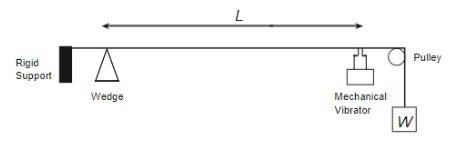
\includegraphics[width=\textwidth]{figures/fig11.jpeg}
    \caption{Apparatus and the arrangement of the experimental setup.}
    \label{fig:yx}
\end{figure}
The experiment is set up as above with the string with and without beads, a signal generator, a speaker that produces waves and weight to create tension in string. 
% Sketch and explain the experimental setup. The explanation should try to cover these pointers:  table 
% \begin{enumerate}
%     \item What is the purpose of individual items in the setup?
%     \item If any equipment is taking measurements, what is it reading and how is it being read?
% \end{enumerate}

% Be precise to, ONLY include scientific description.

\section{Method / Procedure}
We first measure the diameter of the string using a micrometer, measure the length of the string using the meter rule. We also find the theoretical values to have a close frequency range for sweep frequency. We find the value of $\mu$ . Output leads of the signal generated to woofer is connected at 10V. Then we sweep the frequency of the signal generator and find the frequency at which standing waves appear. We do it for the first harmonic, second harmonic, third harmonic, fourth harmonic. We then repeat the same process for the loaded string, with beads, and measure the inter-bead distance first. We find the four harmonic frequencies in the same manner. We note down all harmonics and plot graph between frequency and number of the harmonics for both. 
% Highlight the following aspects of the experiment conducted 
% \begin{enumerate}
%     \item What method did you use to perform the experiment?
%     \item What adjustments were made, if any? 
%     \item What data was collected?
%     \item How was it collected?
%     \item Were any calibrations made and what were they?
% \end{enumerate}

% Be precise to, ONLY include scientific background.

\section{Data}
Type B uncertainty of diameter is 0.00002m and 0.002m for length and 0.002 for frequency. 

\begin{center}
\begin{tabular}{|c|c|c|c|c|}
\hline
\multicolumn{5}{|c|}{\textbf{un-loaded Steel String}} \\ \hline
       & h1        & h2        & h3        & h4       \\ \hline
S.no   & f1 (Hz)   & f2 (Hz)   & f3  (Hz)  & f4 (Hz)  \\ \hline
1      & 23.5      & 46.3      & 70.2      & 95.6     \\ \hline
2      & 24.14     & 50        & 73        & 93       \\ \hline
3      & 23.5      & 46        & 70.8      & 96       \\ \hline
\end{tabular}
\end{center}

\begin{center}
\begin{tabular}{|l|l|}
\hline
\multicolumn{2}{|c|}{\textbf{un-loaded Steel String}} \\ \hline
No. of Anti   Nodes      & Average Frequency(Hz)      \\ \hline
h1                       & 23.71333333                \\ \hline
h2                       & 47.43333333                \\ \hline
h3                       & 71.33333333                \\ \hline
h4                       & 94.86666667                \\ \hline
\end{tabular}
\end{center}

\begin{center}
\begin{tabular}{|c|c|c|c|c|}
\hline
\multicolumn{5}{|c|}{\textbf{Loaded Steel String}} \\ \hline
      & h1       & h2       & h3        & h4       \\ \hline
S.no  & f1 (Hz)  & f2 (Hz)  & f3  (Hz)  & f4 (Hz)  \\ \hline
1     & 13       & 26       & 35        & 44       \\ \hline
2     & 14       & 25       & 35        & 44       \\ \hline
3     & 12.7     & 24.5     & 35.6      & 44.5     \\ \hline
\end{tabular}
\end{center}


\begin{center}
\begin{tabular}{|l|l|}
\hline
\multicolumn{2}{|c|}{\textbf{Loaded Steel String}} \\ \hline
No. of Anti   Nodes     & Average Frequency(Hz)    \\ \hline
h1                      & 13.23333333              \\ \hline
h2                      & 25.16666667              \\ \hline
h3                      & 35.2                     \\ \hline
h4                      & 44.16666667              \\ \hline
\end{tabular}
\end{center}


% In this section, describe what data was recorded during the experiment. Mention which quantities are being measured, which quantity is independent, which is dependent and which are constants. Make this difference very explicit. Make sure to quantify and state the uncertainties in the recorded data. Be precise and primarily include numerical data.

\section{Data Analysis}
We have two equations for density and $\mu$ $$\rho = \frac{mass}{volume}$$ $$\mu =\frac{mass}{l}$$
We equate the two equations according to mass $$\rho * v = l *\mu$$ where v denotes volume and l denotes length. 
It is further divided into 
$$\rho * 2 \pi r^2 * l= l * \mu$$
We get our final equation as $$\mu = \rho * 2 \pi r^2 $$
Our values of tension T and $\mu $ are 11.9878 and 0.00314. 
Our theoretical values for harmonics are calculated using 
\begin{equation}
    f_n = \frac{n}{2L} \sqrt{\frac{T}{\mu}}
\end{equation}
 are as following: 
\begin{center}
\begin{tabular}{|l|l|}
\hline
\multicolumn{2}{|c|}{\textbf{un-loaded Steel String}} \\ \hline
No. of Anti   Nodes          & Frequency(Hz)          \\ \hline
h1                           & 16.96705               \\ \hline
h2                           & 33.9341                \\ \hline
h3                           & 50.90116               \\ \hline
h4                           & 67.86821               \\ \hline
\end{tabular}
\end{center}
\\
For loaded string we calculated harmonics using 
\begin{equation}
    f_n = \frac{n}{2(N+1)m} \sqrt{\frac{T}{\mu}}
\end{equation}
\begin{center}
\begin{tabular}{|l|l|}
\hline
\multicolumn{2}{|c|}{\textbf{Loaded Steel String}} \\ \hline
No. of Anti   Nodes         & Frequency(Hz)        \\ \hline
h1                          & 22.0571682           \\ \hline
h2                          & 44.11433639          \\ \hline
h3                          & 66.17150459          \\ \hline
h4                          & 88.22867278          \\ \hline
\end{tabular}
\end{center}

\newpage
\begin{figure}[h!]
   \centering
    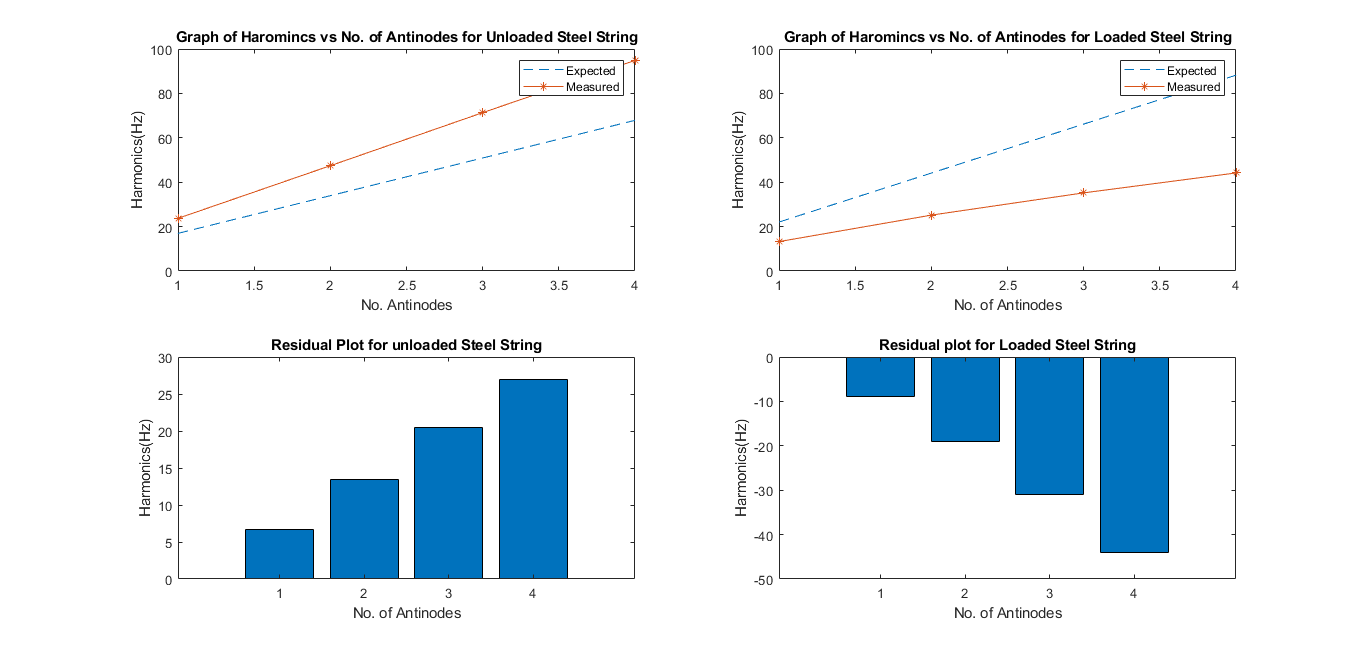
\includegraphics[width=\textwidth]{figures/SubplotsExp12.png}
    \caption{Apparatus and the arrangement of the experimental setup.}
    \label{fig:yx}
\end{figure}

% In this section, mention the calculations you perform, uncertainties transferred, and statistical analysis (residuals, errors, uncertainties in parameters fit etc.). Be precise and primarily include numerical data \ref{eq:line}.

% \begin{figure}[h!]
%     \centering
%     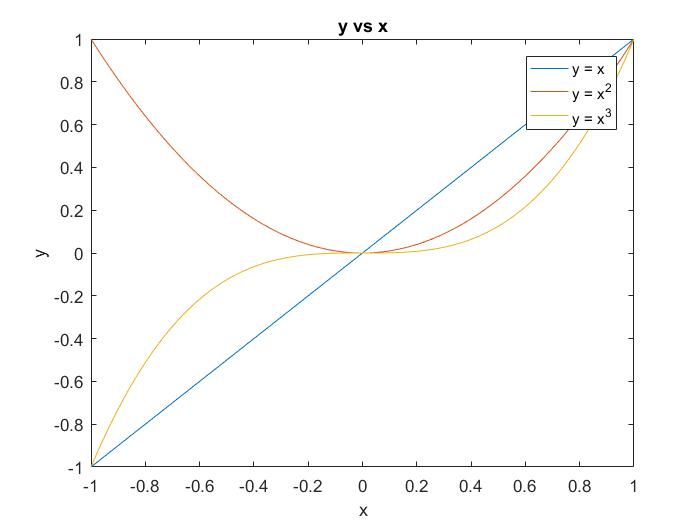
\includegraphics[width=\textwidth]{figures/test.jpg}
%     \caption{Graph of y vs x}
%     \label{fig:yx}
% \end{figure}

\section{Discussion \& Conclusion}

We can see in the graph of Harmonics vs antinodes that there is a linear trend although, the value of harmonics does not double when the number of antinodes increase. Furthermore, we can see from both the residual plots that as the number of antinodes the error in the values of the harmonics also increase. This was expected because as the number of antinodes increase, the maximum amplitude decreases which in turn makes it difficult to observe.  We can reduce the random errors in this experiment by recording more values of harmonics for each antinodes. We can also vary the tension in string using different weights and then repeating the experiment for each value of Tension.

\section{MATLAB Script}
\lstinputlisting{matlabCodes/Experiment12.m}



